\chapter{Evaluation Design}\label{C:ed}
In this chapter we present our performance evaluation of our graph database based approach, by comparing it with an existing approach, namely, the GraphEvol approach presented in \cite{2}. In particular, we evaluated the effectiveness and efficiency of our approach by comparing the quality of composition solutions and the time taken to generate a Web service composition. 

\section{Datasets and Parameters} 
We evaluated the performance of our approach by testing it on a benchmark dataset, WSC2008 \cite{12} which contains service collections of varying sizes. To provide a comparison with the GraphEvol approach, we ran each task independently 30 times, for each run recording the best Web service composition, fitness value and execution time. For all tests we set the weights for an objective function to the same value as was used with the GraphEvol method, namely, a fixed weight of 0.25. The other parameters for GraphEvol were: a population of 200 candidates, a mutation probability of 0.05, and a crossover probability of 0.5. Individuals were chosen for breeding using tournament selection with a tournament size of 2 \cite{2}.\par

The test to compare the performance of the graph database approach and GraphEvol approach is conducted on a Macbook Pro Mid 2012 with a 2.9GHz dual-core Intel Core i7 processor, 8GB of 1600MHz DDR3 memory, a 1536 Mb Intel HD Graphics 4000 graphics card, a 128GB solid-state drive and the OS X EI Capitan operating system.

\section{Evaluation Results} 
In this section we present the results of our evaluation of our proposed algorithms. 

\subsection{Effectiveness of the Reducing Algorithm} 
To evaluate the effectiveness of our reducing graph database algorithm we applied it to all test cases contained of WSC2008 \cite{12}.  Table \ref{tb:reduce} shows the number of Web services for the original repositories and the number of Web service for the reduced graph database. For example, for WSC2008-02, there were 558 Web services in the original repository, but only 66 of them were related to the task input and task output. For task WSC2008-08, there were 8138 Web service in the original repository, but only 131 of them were related to the task input and output. Thus, the number of the Web services was greatly reduced when compared to the number in the original repositories, which greatly improved the execution time when generating the Web service composition.

\begin{table}[]
\centering
\caption{Comparison of the number of services in the original repositories and the reduced repositories}
\label{tb:reduce}
\scalebox{0.9}{

\begin{tabular}{|c|c|c|ll}
\cline{1-3}
Dataset WSC2008 & Original service repository & Reduced Service repository &  &  \\ \cline{1-3}
01              & 158                         & 61                         &  &  \\ \cline{1-3}
02              & 558                         & 66                         &  &  \\ \cline{1-3}
03              & 604                         & 105                        &  &  \\ \cline{1-3}
04              & 1041                        & 46                         &  &  \\ \cline{1-3}
05              & 1091                        & 102                        &  &  \\ \cline{1-3}
06              & 2198                        & 205                        &  &  \\ \cline{1-3}
07              & 4113                        & 195                        &  &  \\ \cline{1-3}
08              & 8119                        & 131                        &  &  \\ \cline{1-3}
\end{tabular}
}
\end{table}

\subsection{Correctness of the Web Service Composition} 
A composition correctness evaluation was carried out to check correctness of the Web service compositions. The correctness of the Web service composition was determined by checking that all the service node inputs are fulfilled by the output of their proceeding nodes in the graph database. We checked the correctness of all the service composition solutions produced by our algorithm. Our evaluation showed that all the solutions were correct. In this report, we show two composition solutions for Task 1 of WSC2008 with a repository of 158 services. The following examples show that for Task 1 the task and the service compositions produced by our approach (see Figure \ref{fig:c4compEg1} and Figure \ref{fig:c4compEg2}).\\

Task 1: \emph{WSC2008-01}\par
Task 1 inputs: \emph{[inst1926141668, inst395151449, inst1557679659]}\par
Task 1 outputs: \emph{[inst1913443608, inst664891780]}\\\par

\begin{figure}[h]
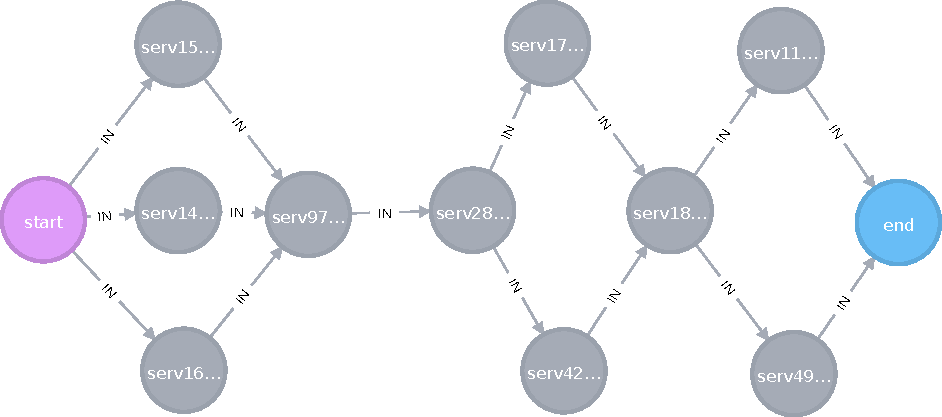
\includegraphics[width=11cm]{svg-chapter4-c1.pdf}
\centering
\caption{Web service composition 1 (Task1, WSC2008-01)}
\label{fig:c4compEg1} 
\end{figure} 
\begin{exmp}
In Figure \ref{fig:c4compEg1}, showing a example of Web service composition, the input of the Web service \emph{serv283321609} is \emph{I} = \emph{{ inst722854357, inst347634243, inst1881697469, inst746203847 }}. This matches the output  \emph{O} = \emph{{inst722854357, inst2092246857, inst1326239605, inst1881697469, inst1437249127, inst1519789560 }} of Web service  \emph{serv976005395}. This exact match occurs as \emph{inst722854357} and \emph{inst1881697469} are found in both Web service \emph{serv283321609} and Web service \emph{serv976005395}, while,  according to the taxonomy tree, \emph{inst1519789560} and \emph{inst1326239605} in \emph{O} are specializations of \emph{inst347634243} in \emph{I} and \emph{inst1437249127} in \emph{O} is a specialization of \emph{inst746203847} in \emph{I}.\par
\end{exmp}

\begin{figure}[h]
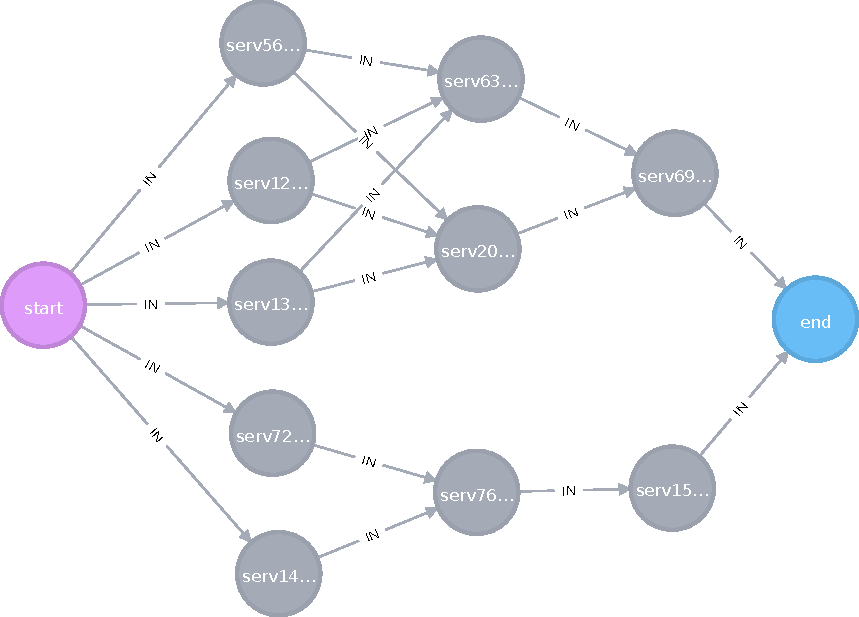
\includegraphics[width=11cm]{svg-chapter4-c2.pdf}
\centering
\caption{Web service composition 2 (Task1, WSC2008-01)}
\label{fig:c4compEg2} 
\end{figure} 

\begin{exmp}
In Figure \ref{fig:c4compEg2},  the input of the web service \emph{serv699915007} is \emph{I} = \emph{{inst102675811, inst1689375842, inst1716616603}}. This matches the output \emph{O$_1$} = \emph{{inst927259823,inst608977925 }} of Web service  \emph{serv2085282617} and the output \emph{O$_2$} = \emph{{inst885068313,inst1420249694,inst1488043421 }} of Web service  \emph{serv630482774}. As you can see there is no exact match between the outputs of services \emph{serv2085282617} and \emph{serv630482774}, and inputs of service \emph{serv699915007}, while, according to the taxonomy tree, \emph{inst1488043421} in \emph{O$_2$} is a specialization of inst102675811 in \emph{I}, \emph{inst927259823} in \emph{O$_1$} is a specialization of \emph{inst1689375842} in \emph{I} and  \emph{inst885068313} in \emph{O$_2$} is a specialization of \emph{inst1716616603} in \emph{I}.\par
\end{exmp}

Thus, the number of Web services involved in both examples is the same. Since we are only evaluating the correctness of the composition, we do not know whether the Web services composition is capable of performing tasks reliably or efficiently (i.e accounting for non-functional attributes). The next section presents the performance of our QoS-aware approach by comparing it with the GraphEvol approach.\par

\subsection{Evaluation Results for QoS-Aware Service Composition} 
Table \ref{tb:evalComp} shows a full evaluation comparing the performance of our approach and that of the  GraphEvol approach \cite{2}. Both approaches were run on the same machine (mentioned in Section 4.1) to conduct significant analyses. We ran each task independently, for each run recording the best Web service composition, the number of services involved, the fitness value and the execution time taken. Then we calculated the mean, standard deviation for the number of services involved, fitness values and execution times separately for each task. For each run, our approach generated \emph{50} candidates and the best solution from those candidates was chosen. For GraphEvol approach, the best candidate was generated from a population size of \emph{200}.\par

Table \ref{tb:evalComp} includes three columns for each approach. The \emph{number} column records the number of services involved in the best Web service composition.  The \emph{time} column records the average time, over 30 independent runs, which was taken to generate the best Web service composition. And the \emph{fitness} column records the average \emph{QoS} fitness value for the best Web service composition, calculated from 30 independent runs.

\begin{table}[h]
\centering
\caption{ Average results of the tests for QoS-aware service composition}
\label{tb:evalComp}
\scalebox{0.66}{
\begin{tabular}{|c|c|c|c|c|c|c|}
\hline
\textbf{Dataset} & \multicolumn{3}{c|}{\textbf{Graph Database Approach}} & \multicolumn{3}{c|}{\textbf{GraphEvol Approach}}  \\ \hline
\textbf{2008}    & \textbf{Number}   & \textbf{Time (ms)}   & \textbf{Fitness}   & \textbf{Number} & \textbf{Time (ms)} & \textbf{Fitness}    \\ \hline
1                & 10 \rlap{{$\pm$}}\hspace{0.4cm} 0.00             & 2197.90 \rlap{{$\pm$}}\hspace{0.4cm}329 \rlap{{$\downarrow$}}          & 0.521 \rlap{{$\pm$}}\hspace{0.4cm}0.169 \rlap{{$\downarrow$}}      & 10.63 \rlap{{$\pm$}}\hspace{0.4cm}2.17      & 4845.57 \rlap{{$\pm$}}\hspace{0.4cm}315.42     & 0.645 \rlap{{$\pm$}}\hspace{0.4cm}0.139                \\ \hline
2                & 5  \rlap{{$\pm$}}\hspace{0.4cm} 0.00               & 5347.13 \rlap{{$\pm$}}\hspace{0.4cm}880 \rlap{{$\uparrow$}}           & 0.48 \rlap{{$\pm$}}\hspace{0.4cm}0.152 \rlap{{$\downarrow$}}        & 5.87 \rlap{{$\pm$}}\hspace{0.4cm}2.12       & 3699.77 \rlap{{$\pm$}}\hspace{0.4cm}364.57     & 0.906 \rlap{{$\pm$}}\hspace{0.4cm}0.00                  \\ \hline
3                & 40 \rlap{{$\pm$}}\hspace{0.4cm} 0.00               & 10961.53 \rlap{{$\pm$}}\hspace{0.4cm}790 \rlap{{$\downarrow$}}         & 0.387 \rlap{{$\pm$}}\hspace{0.4cm}0.1 \rlap{{$\uparrow$}}         & 41.2 \rlap{{$\pm$}}\hspace{0.4cm}0.79       & 17221.53 \rlap{{$\pm$}}\hspace{0.4cm}764.85    & 0.176 \rlap{{$\pm$}}\hspace{0.4cm}0.045           \\ \hline
4                & 10 \rlap{{$\pm$}}\hspace{0.4cm} 0.00              & 3885.70 \rlap{{$\pm$}}\hspace{0.4cm}399 \rlap{{$\downarrow$}}          & 0.431 \rlap{{$\pm$}}\hspace{0.4cm}0.066 \rlap{{$\uparrow$}}       & 10.2 \rlap{{$\pm$}}\hspace{0.4cm}0.48       & 6076.7 \rlap{{$\pm$}}\hspace{0.4cm}281.58      & 0.305 \rlap{{$\pm$}}\hspace{0.4cm}0.066            \\ \hline
5                & 20 \rlap{{$\pm$}}\hspace{0.4cm} 0.00             & 4510.6 \rlap{{$\pm$}}\hspace{0.4cm}468 \rlap{{$\downarrow$}}           & 0.403 \rlap{{$\pm$}}\hspace{0.4cm}0.128\rlap{{$\uparrow$}}        & 22.13 \rlap{{$\pm$}}\hspace{0.4cm}2.59      & 10444.2 \rlap{{$\pm$}}\hspace{0.4cm}572.59     & 0.164 \rlap{{$\pm$}}\hspace{0.4cm}0.046            \\ \hline
6                & 40 \rlap{{$\pm$}}\hspace{0.4cm} 0.00              & 258503.33 \rlap{{$\pm$}}\hspace{0.4cm}42324 \rlap{{$\uparrow$}}       & 0.407 \rlap{{$\pm$}}\hspace{0.4cm}0.089 \rlap{{$\uparrow$}}       & 40.2 \rlap{{$\pm$}}\hspace{0.4cm}0.48       & 22183.53 \rlap{{$\pm$}}\hspace{0.4cm}1639      & 0.228 \rlap{{$\pm$}}\hspace{0.4cm}0.06           \\ \hline
7                & 20 \rlap{{$\pm$}}\hspace{0.4cm} 0.00              & 17839.77 \rlap{{$\pm$}}\hspace{0.4cm}763 \rlap{{$\downarrow$}}          & 0.457 \rlap{{$\pm$}}\hspace{0.4cm}0.097 \rlap{{$\uparrow$}}       & 23.13 \rlap{{$\pm$}}\hspace{0.4cm}7.33      & 20304.37 \rlap{{$\pm$}}\hspace{0.4cm}1257      & 0.316 \rlap{{$\pm$}}\hspace{0.4cm}0.039          \\ \hline
8                & 30 \rlap{{$\pm$}}\hspace{0.4cm} 0.00              & 53003.7 \rlap{{$\pm$}}\hspace{0.4cm}4465 \rlap{{$\uparrow$}}          & 0.468 \rlap{{$\pm$}}\hspace{0.4cm}0.091 \rlap{{$\uparrow$}}       & 32.47 \rlap{{$\pm$}}\hspace{0.4cm}3.86      & 18567.03 \rlap{{$\pm$}}\hspace{0.4cm}2055      & 0.315 \rlap{{$\pm$}}\hspace{0.4cm}0.028                \\ \hline
\end{tabular}
}
\end{table}

% \begin{table}[h]
% \centering
% \caption{ Average results of the tests for QoS-Aware service composition}
% \label{tb:evalComp}
% \scalebox{0.66}{
% \begin{tabular}{|c|c|c|c|c|c|c|c|c|}
% \hline
% \textbf{Dataset} & \multicolumn{3}{c|}{\textbf{Graph Database (Neo4j) Approach}} & \multicolumn{3}{c|}{\textbf{GraphEvol Approach}}        & \multicolumn{2}{c|}{\textbf{T-Test P value}} \\ \hline
% \textbf{2008}    & \textbf{Number}   & \textbf{Time (ms)}   & \textbf{Fitness}   & \textbf{Number} & \textbf{Time (ms)} & \textbf{Fitness} & \textbf{Fitness}       & \textbf{Time}       \\ \hline
% 1                & 10 \rlap{{$\pm$}}\hspace{0.4cm} 0.00             & 2197.90 \rlap{{$\pm$}}\hspace{0.4cm}329 \rlap{{$\downarrow$}}          & 0.521 \rlap{{$\pm$}}\hspace{0.4cm}0.169       & 10.63 \rlap{{$\pm$}}\hspace{0.4cm}2.17      & 4845.57 \rlap{{$\pm$}}\hspace{0.4cm}315.42     & 0.645 \rlap{{$\pm$}}\hspace{0.4cm}0.139      & 0.999                  & 6.96E-38            \\ \hline
% 2                & 5  \rlap{{$\pm$}}\hspace{0.4cm} 0.00               & 5347.13 \rlap{{$\pm$}}\hspace{0.4cm}880           & 0.48 \rlap{{$\pm$}}\hspace{0.4cm}0.152         & 5.87 \rlap{{$\pm$}}\hspace{0.4cm}2.12       & 3699.77 \rlap{{$\pm$}}\hspace{0.4cm}364.57     & 0.906 \rlap{{$\pm$}}\hspace{0.4cm}0.00       & 0.9999                 & 0.99999             \\ \hline
% 3                & 40 \rlap{{$\pm$}}\hspace{0.4cm} 0.00               & 10961.53 \rlap{{$\pm$}}\hspace{0.4cm}790 \rlap{{$\downarrow$}}         & 0.387 \rlap{{$\pm$}}\hspace{0.4cm}0.1 \rlap{{$\uparrow$}}         & 41.2 \rlap{{$\pm$}}\hspace{0.4cm}0.79       & 17221.53 \rlap{{$\pm$}}\hspace{0.4cm}764.85    & 0.176 \rlap{{$\pm$}}\hspace{0.4cm}0.045      & 2.38E-13               & 2.06E-37            \\ \hline
% 4                & 10 \rlap{{$\pm$}}\hspace{0.4cm} 0.00              & 3885.70 \rlap{{$\pm$}}\hspace{0.4cm}399 \rlap{{$\downarrow$}}          & 0.431 \rlap{{$\pm$}}\hspace{0.4cm}0.066 \rlap{{$\uparrow$}}       & 10.2 \rlap{{$\pm$}}\hspace{0.4cm}0.48       & 6076.7 \rlap{{$\pm$}}\hspace{0.4cm}281.58      & 0.305 \rlap{{$\pm$}}\hspace{0.4cm}0.066      & 5.58E-110              & 3.03E-30            \\ \hline
% 5                & 20 \rlap{{$\pm$}}\hspace{0.4cm} 0.00             & 4510.6 \rlap{{$\pm$}}\hspace{0.4cm}468 \rlap{{$\downarrow$}}           & 0.403 \rlap{{$\pm$}}\hspace{0.4cm}0.128\rlap{{$\uparrow$}}        & 22.13 \rlap{{$\pm$}}\hspace{0.4cm}2.59      & 10444.2 \rlap{{$\pm$}}\hspace{0.4cm}572.59     & 0.164 \rlap{{$\pm$}}\hspace{0.4cm}0.046      & 8.80E-12               & 1.95E-44            \\ \hline
% 6                & 40 \rlap{{$\pm$}}\hspace{0.4cm} 0.00              & 258503.33 \rlap{{$\pm$}}\hspace{0.4cm}42324      & 0.407 \rlap{{$\pm$}}\hspace{0.4cm}0.089 \rlap{{$\uparrow$}}       & 40.2 \rlap{{$\pm$}}\hspace{0.4cm}0.48       & 22183.53 \rlap{{$\pm$}}\hspace{0.4cm}1639      & 0.228 \rlap{{$\pm$}}\hspace{0.4cm}0.06       & 1.81E-12               & 1.0                   \\ \hline
% 7                & 20 \rlap{{$\pm$}}\hspace{0.4cm} 0.00              & 17839.77 \rlap{{$\pm$}}\hspace{0.4cm}763 \rlap{{$\downarrow$}}          & 0.457 \rlap{{$\pm$}}\hspace{0.4cm}0.097 \rlap{{$\uparrow$}}       & 23.13 \rlap{{$\pm$}}\hspace{0.4cm}7.33      & 20304.37 \rlap{{$\pm$}}\hspace{0.4cm}1257      & 0.316 \rlap{{$\pm$}}\hspace{0.4cm}0.039      & 3.83E-09               & 3.98E-12            \\ \hline
% 8                & 30 \rlap{{$\pm$}}\hspace{0.4cm} 0.00              & 53003.7 \rlap{{$\pm$}}\hspace{0.4cm}4465         & 0.468 \rlap{{$\pm$}}\hspace{0.4cm}0.091 \rlap{{$\uparrow$}}       & 32.47 \rlap{{$\pm$}}\hspace{0.4cm}3.86      & 18567.03 \rlap{{$\pm$}}\hspace{0.4cm}2055      & 0.315 \rlap{{$\pm$}}\hspace{0.4cm}0.028      & 1.44E-10               & 1.0                   \\ \hline
% \end{tabular}
% }
% \end{table}

\subsubsection{The number of the Web services involved} 

The results in Table \ref{tb:servSize} compare the number of Web services required for a composition using two approaches. The result (number of services invoked) with the {'}\emph{minimum number of Web services}{'} approach was equal to or very close to the result using the {'}\emph{non-minimum number of Web services}{'} approach. However, the fitness values were much higher with the {'}\emph{minimum number of Web services}{'} approach. A poor result occurred with Datasets \emph{1} and \emph{3}, and with Dataset \emph{3} the {'}\emph{non-minimum number of Web services}{'} approach took \emph{1138667.65} milliseconds (\emph{19} minutes) to generate a single service composition due to the huge search space involved, compared with \emph{10916.53} milliseconds (\emph{10.9} seconds) using the the {'}\emph{minimum number of Web services}{'} method. This was because when we restrict our approach to a minimum number of Web services, the search space is also restricted. The result was that when we added web service nodes into the service composition, whenever the number of the web services in the composition was greater than the minimum number of the Web services, our approach led to continual re-starting of the composition generation step in order to find a new composition.\par

So we decided to use the {'}\emph{minimum number of Web services}{'} method to generate Web service compositions in order to find the best candidates. The result was that the number of the services involved in our approach was less than or equal to the numbers of services when using the GraphEvol approach.\par

\subsubsection{Execution time to generate best QoS-Aware Web service composition} 
Our approach successfully generated a Web service composition for each task in eight datasets from WSC2008. For five tasks our approach was significantly better than the GraphEvol approach in terms of execution time. However, the composition generation time for the remaining three tasks was slower than when using the GraphEvol approach. This was especially true for Dataset \emph{6}, which took \emph{258503.33} milliseconds using our approach compared with \emph{22183.53} milliseconds using the GraphEvol approach.\par

The result we obtained when using our algorithm with Dataset \emph{6} occurred because Dataset \emph{6} required \emph{40} Web service nodes for the composition and the reduced graph database contained \emph{205} Web service nodes. So one of five nodes was involved in the composition leading to a large number of edges (relationships) between the Web service nodes, and the large number of service nodes and edges increased the search space, thus increasing the total execution time in generating a composition. But overall, our approach performed better than the GraphEvol approach and led to faster generation of web compositions.\par



\begin{table}[h]
\centering
\caption{ Graph Database: Average (30 independent runs) results}
\label{tb:servSize}
\scalebox{0.8}{
\begin{tabular}{|c|c|c|c|c|c|c|}
\hline
Dataset & \multicolumn{3}{c|}{Using minimum number of services} & \multicolumn{3}{c|}{Using non-minimum number of  services} \\ \hline
2008    & Number        & Time (ms)          & Fitness          & Number            & Time (ms)           & Fitness          \\ \hline
1       & 10 \rlap{{$\pm$}}\hspace{0.4cm} 0.00            & 2197.90 \rlap{{$\pm$}}\hspace{0.4cm} 329  \rlap{{$\uparrow$}}       & 0.52\rlap{{$\pm$}}\hspace{0.4cm}0.166        & 10 \rlap{{$\pm$}}\hspace{0.4cm} 0.00               & 1047.06 \rlap{{$\pm$}}\hspace{0.4cm} 367          & 0.53 \rlap{{$\pm$}}\hspace{0.4cm} 0.174        \\ \hline
2       & 5 \rlap{{$\pm$}}\hspace{0.4cm} 0.00           & 5347.13\rlap{{$\pm$}}\hspace{0.4cm}880  \rlap{{$\uparrow$}}      & 0.54\rlap{{$\pm$}}\hspace{0.4cm}0.103        & 5 \rlap{{$\pm$}}\hspace{0.4cm} 0.00                & 3699.77\rlap{{$\pm$}}\hspace{0.4cm}364.57       & 0.546\rlap{{$\pm$}}\hspace{0.4cm}0.179       \\ \hline
4       & 10 \rlap{{$\pm$}}\hspace{0.4cm} 0.00           & 3885.70\rlap{{$\pm$}}\hspace{0.4cm}399  \rlap{{$\downarrow$}}       & 0.388\rlap{{$\pm$}}\hspace{0.4cm}0.08       & 10 \rlap{{$\pm$}}\hspace{0.4cm} 0.00               & 6076.7\rlap{{$\pm$}}\hspace{0.4cm}281.58        & 0.26\rlap{{$\pm$}}\hspace{0.4cm}0.028        \\ \hline
3       & 40 \rlap{{$\pm$}}\hspace{0.4cm} 0.00           & 10961.53\rlap{{$\pm$}}\hspace{0.4cm}790 \rlap{{$\downarrow$}}        & 0.387\rlap{{$\pm$}}\hspace{0.4cm}0.1        & 40 \rlap{{$\pm$}}\hspace{0.4cm} 0.00                 & 1138667.65 \rlap{{$\pm$}}\hspace{0.4cm}83582.58                 & 0.211\rlap{{$\pm$}}\hspace{0.4cm}0.068               \\ \hline
5       & 20 \rlap{{$\pm$}}\hspace{0.4cm} 0.00           & 4510.6\rlap{{$\pm$}}\hspace{0.4cm}468  \rlap{{$\downarrow$}}       & 0.398\rlap{{$\pm$}}\hspace{0.4cm}0.121      & 20 \rlap{{$\pm$}}\hspace{0.4cm} 0.00               & 10444.2\rlap{{$\pm$}}\hspace{0.4cm}572.59       & 0.227\rlap{{$\pm$}}\hspace{0.4cm}0.065       \\ \hline
6       & 40 \rlap{{$\pm$}}\hspace{0.4cm} 0.00           & 258503.33\rlap{{$\pm$}}\hspace{0.4cm}42324 \rlap{{$\uparrow$}}      & 0.354\rlap{{$\pm$}}\hspace{0.4cm}0.103       & 42.067\rlap{{$\pm$}}\hspace{0.4cm}1.29        & 22183.53\rlap{{$\pm$}}\hspace{0.4cm}1639         & 0.206\rlap{{$\pm$}}\hspace{0.4cm}0.086       \\ \hline
7       & 20 \rlap{{$\pm$}}\hspace{0.4cm} 0.00           & 17839.77\rlap{{$\pm$}}\hspace{0.4cm}763  \rlap{{$\downarrow$}}     & 0.411\rlap{{$\pm$}}\hspace{0.4cm}0.076      & 20 \rlap{{$\pm$}}\hspace{0.4cm} 0.00               & 20304.37\rlap{{$\pm$}}\hspace{0.4cm}1257         & 0.317\rlap{{$\pm$}}\hspace{0.4cm}0.085       \\ \hline
8       & 30 \rlap{{$\pm$}}\hspace{0.4cm} 0.00           & 53003.7\rlap{{$\pm$}}\hspace{0.4cm}4465  \rlap{{$\downarrow$}}     & 0.438\rlap{{$\pm$}}\hspace{0.4cm}0.012      & 33.67\rlap{{$\pm$}}\hspace{0.4cm}2.29         & 284831.37\rlap{{$\pm$}}\hspace{0.4cm}2125         & 0.358\rlap{{$\pm$}}\hspace{0.4cm}0.052       \\ \hline
\end{tabular}
}
\end{table}

\subsubsection{Hypothesis test using two fitness value sets for each approach} 

We used a two-sample t-test to check if the fitness values and execution times for our approach were better than the fitness values and execution times for the GraphEvol approach at the \emph{0.05} significance level. In Table \ref{tb:evalComp}, it is clear that the P-values from datasets \emph{03} to \emph{08} are smaller than the significance level \emph{0.05} for the fitness values set and Datasets \emph{1, 3, 4, 5} and \emph{7} are less than the significance level \emph{0.05} for the execution times set, as indicated by the upward and downward pointing arrows. This means there is considerable evidence that the sets of fitness values and execution times for GraphEvol approach are lower than for our approach. In other words, the best solutions in our approach are significantly superior to the best solutions produced by the GraphEvol approach for 6 out of 8 tasks. For execution time, our approach are faster than GraphEvol for 5 out of 8 tasks and only with Dataset \emph{2, 6} and \emph{8} were our execution time sets poorer than with the GraphEvol approach. In summary however, our approach successfully produced a better result overall, than the GraphEvol approach, in most test cases using the benchmark dataset.\par

\subsection{Summary}
This chapter we evaluate  the performance of our proposed graph database-based approach with an existing GP-based approach by comparing with an existing GP-based approach known as GraphEvol, which is presented in \cite{2}. From our evaluation results, we can conclude that our approach is efficient and effective in generating service composition solutions. It can generate near-optimal QoS-aware composition solutions in a shorter time than the GraphEvol approach.